% Copyright 2004 by Till Tantau <tantau@users.sourceforge.net>.
%
% In principle, this file can be redistributed and/or modified under
% the terms of the GNU Public License, version 2.
%
% However, this file is supposed to be a template to be modified
% for your own needs. For this reason, if you use this file as a
% template and not specifically distribute it as part of a another
% package/program, I grant the extra permission to freely copy and
% modify this file as you see fit and even to delete this copyright
% notice. 

\documentclass{beamer}
\usepackage[utf8]{inputenc}
\usepackage[brazilian]{babel}

% There are many different themes available for Beamer. A comprehensive
% list with examples is given here:
% http://deic.uab.es/~iblanes/beamer_gallery/index_by_theme.html
% You can uncomment the themes below if you would like to use a different
% one:
%\usetheme{AnnArbor}
%\usetheme{Antibes}
%\usetheme{Bergen}
%\usetheme{Berkeley}
%\usetheme{Berlin}
%\usetheme{Boadilla}
%\usetheme{boxes}
\usetheme{CambridgeUS}
%\usetheme{Copenhagen}
%\usetheme{Darmstadt}
%\usetheme{default}
%\usetheme{Frankfurt}
%\usetheme{Goettingen}
%\usetheme{Hannover}
%\usetheme{Ilmenau}
%\usetheme{JuanLesPins}
%\usetheme{Luebeck}
%\usetheme{Madrid}
%\usetheme{Malmoe}
%\usetheme{Marburg}
%\usetheme{Montpellier}
%\usetheme{PaloAlto}
%\usetheme{Pittsburgh}
%\usetheme{Rochester}
%\usetheme{Singapore}
%\usetheme{Szeged}
%\usetheme{Warsaw}

\title{Aula 2 - Unix}

% A subtitle is optional and this may be deleted
\subtitle{Curso de Unix}

\author{PET Computa\c{c}ão}
% - Give the names in the same order as the appear in the paper.
% - Use the \inst{?} command only if the authors have different
%   affiliation.

\institute[UFSC] % (optional, but mostly needed)
{
%
  Departamento de Informática e Estatística\\
  Universidade de Santa Catarina}
% - Use the \inst command only if there are several affiliations.
% - Keep it simple, no one is interested in your street address.

\date{PET Computa\c{c}ão, 2015}
% - Either use conference name or its abbreviation.
% - Not really informative to the audience, more for people (including
%   yourself) who are reading the slides online

\subject{Curso de Unix}
% This is only inserted into the PDF information catalog. Can be left
% out. 

% If you have a file called "university-logo-filename.xxx", where xxx
% is a graphic format that can be processed by latex or pdflatex,
% resp., then you can add a logo as follows:

% \pgfdeclareimage[height=0.5cm]{university-logo}{university-logo-filename}
% \logo{\pgfuseimage{university-logo}}

% Delete this, if you do not want the table of contents to pop up at
% the beginning of each subsection:
\AtBeginSubsection[]
{
  \begin{frame}<beamer>{Sumário}
    \tableofcontents[currentsection,currentsubsection]
  \end{frame}
}

% Let's get started
\begin{document}

\begin{frame}
  \titlepage
\end{frame}

\begin{frame}{Sumário}
  \tableofcontents
  % You might wish to add the option [pausesections]
\end{frame}

% Section and subsections will appear in the presentation overview
% and table of contents.
\section{Trabalhando com arquivos}

\subsection{cp (copy)}

\begin{frame}{Copiando arqiuvos}{cp (copy)}
  \begin{itemize}
  \item {
    Utilizando o comando \textbf{cp arquivo1 arquivo2} você cria uma cópia do \textit{arquivo1} e a chama de \textit{arquivo2}.
  }
  \end{itemize}
    \begin{figure}[h!]
        \centering
        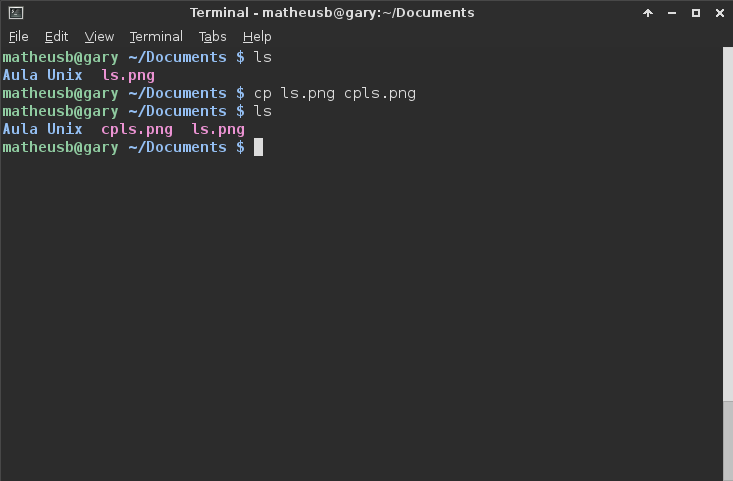
\includegraphics[scale=0.30]{cp.png}
        \caption{Comando ls}
        \label{fig:Comando ls}
    \end{figure}
\end{frame}

\subsection{mv (move)}
\begin{frame}{Movendo arqiuvos}{mv (move)}
  \begin{itemize}
  \item {
    O comando mv possui duas fun\c{c}ões bem semelhantes.
    } 
    \item{ \textbf{mv arquivo1 arquivo2} desta forma você modifica o \textit{arquivo1} e o chama de \textit{arquivo2}.
    }
    \item{Você pode também utilizar ele para mover o arquivo de um diretório para o outro, desta forma: \textbf{mv arquivo1 diretorio}.
  }
  \end{itemize}
\end{frame}

\subsection{rm (remove)}
\begin{frame}{Removendo arquivos}{rm (remove)}
  \begin{itemize}
  \item {
    O comando rm é o comando básico de remoção de arquivos do Linux
    } 
    \item{ \textbf{rm arquivo1} Desta forma você apaga o \textbf{arquivo1}.
    }
    \item{Você pode também utilizar ele para remover um diretório, usando a flag -r, \textbf{rm -r diretorio}.
  }
 
  \end{itemize}
\end{frame}


\subsection{cat (concatenate) e clear}
\begin{frame}{Concatenar}{cat (concatenate) e clear}
  \begin{itemize}
  \item {   O comando cat (concatenar) pode ser usado para mostrar o conteúdo de arquivos no terminal.
   } 
    \item{ \textbf{cat arquivo1} desta forma você exibe o conteúdo do \textit{arquivo1} no terminal 
    }
    \item{Você pode também utilizar ele para exibir o conteúdo de dois ou mais arquivos \textbf{concatenados}, \textbf{cat arquivo1 arquivo2}.
    \item{Após utilizar o comando cat, você poderá desejar "limpar" o seu terminal, para isto use o comando \textbf{clear} ele apagara todos os comandos escritos no terminal e seus retornos, deixando o terminal como recém aberto.}
  }
  \end{itemize}
\end{frame}

\section*{Sumário dos comandos}

\begin{frame}{Sumário dos comandos}
 \begin{center}
 \begin{tabular}{||c | c||} 
 \hline
 \textbf{Comando} & \textbf{Descri\c{c}ão}\\ [0.5ex] 
 \hline\hline
 cp & Copia o arquivo fonte para o destino\\ 
 \hline
 mv & move o um arquivo para outro arquivo ou diretório\\
 \hline
 rm & remove o arquivo, com a flag \textbf{-r} remove o diretório\\
 \hline
 cat & mostra o conteúdo dos arquivos no terminal \\
 \hline
 clear & limpa todos os comandos e retornos escritos no terminal\\
 \hline
\end{tabular}
\end{center}
\end{frame}
\end{document}


